\documentclass[aspectratio=169]{beamer}
   \usetheme[subsectionpage=progressbar]{metropolis}
   \setbeamertemplate{blocks}[rounded][shadow=false]
\usepackage{url}
\usepackage{hyperref}
\usepackage{booktabs}
\usepackage{tabularx}
\usepackage{dcolumn}
   \newcolumntype{d}[1]{D{.}{.}{#1}}
\usepackage{graphicx}
\usepackage[justification=raggedright]{caption}
\usepackage{adjustbox}
\usepackage{color}
\usepackage[super]{nth}
\usepackage{textpos}
\usepackage{etoolbox}
\usepackage{tcolorbox}
\usepackage{multimedia}
\usepackage{comment}
\usepackage{pgfpages}

\captionsetup[figure]{justification=centering}

\makeatletter
\patchcmd{\beamer@sectionintoc}{\vskip1.5em}{\vskip0.5em}{}{}
\makeatother

\definecolor{smured}{rgb}{0.797,0,0.027}
\definecolor{smublue}{RGB}{48,64,116}
\definecolor{dkgreen}{rgb}{0,0.6,0}
\definecolor{gray}{rgb}{0.5,0.5,0.5}
\definecolor{mauve}{rgb}{0.58,0,0.82}
\definecolor{text_gray}{RGB}{46,58,62}

\setbeamercolor{progress bar}{fg=smured,bg=smublue}
\setbeamercolor{title separator}{fg=smublue}
\setbeamercolor{frametitle}{bg=smublue}

\newtcolorbox{mybox}{colback=smublue,colframe=smublue!75!black}

\metroset{
  numbering=fraction
}

\hypersetup{
  colorlinks=true,
  allcolors=text_gray,
  urlcolor=smured,
}

\addtobeamertemplate{frametitle}{}{
\begin{textblock*}{1cm}(\textwidth,-0.96cm)

\includegraphics[width=0.9cm]{images/smu_logo.pdf}
\end{textblock*}}

%\setbeameroption{show notes on second screen}
%\setbeamertemplate{note page}{%
%  \insertnote%
%}
\setbeamercolor{alerted text}{fg=smured}

\title{ColdFront Town Hall}
\institute{
O'Donnell Data Science and Research Computing Institute\\
SMU}
\date{}

\begin{document}

\begin{frame}
\titlepage
\end{frame}

\begin{frame}{Outline}
\footnotesize
\tableofcontents[hideallsubsections]
\end{frame}

\section{Introductions}

\begin{frame}{O'Donnell Data Science and Research Computing Institute}
\begin{itemize}
\item Dr. Neena Imam, \textit{Peter O'Donnell Jr. Director}
\item Dr. Robert Kalescky, \textit{Principal Scientist}
\end{itemize}
\end{frame}

\begin{frame}{OIT}
\begin{itemize}
\item Project Management
\begin{itemize}
\item Rachel Mulry, \textit{Associate CIO for Planning and Customer Service}
\item Shanta Ball, \textit{Associate Project Manager}
\end{itemize}
\item Data Center and HPC
\begin{itemize}
\item John Patterson, \textit{Director of Data Center and HPC}
\item Amit Kumar, \textit{Information Technology Architect}
\item Richard England, \textit{Sr. Systems Administrator}
\end{itemize}
\item Research Technology Services
\begin{itemize}
\item Dr. Eric Godat, \textit{Director of OIT Research Technology Services}
\item Dr. John LaGrone, \textit{HPC Research Solutions Architect}
\end{itemize}
\end{itemize}
\end{frame}

\section{ColdFront}

% Overview
% What it is...
% Why we're using it...
% How to use it (outline)...
% Support resources...

\begin{frame}{Overview}
\small
\begin{columns}[c]
\begin{column}{0.5\textwidth}
\begin{itemize}
\item<1-| alert@1> ColdFront is an application that helps manage HPC resource
allocations
\item<2-| alert@2> Allows authorized individuals to:
\begin{itemize}
\item<3-| alert@3> Manage projects
\item<4-| alert@4> Request compute resources
\item<5-| alert@5> Request storage resources
\item<6-| alert@6> Assign user access permissions
\end{itemize}
\item<7-| alert@7> Provisioning is automated
\end{itemize}
\end{column}
\begin{column}{0.5\textwidth}
\centering
\frame{
\includegraphics[width=0.85\textwidth]{images/cf_logo.jpeg}}
\end{column}
\end{columns}
\end{frame}

\begin{frame}{Benefits}
\small
\begin{columns}[c]
\begin{column}{0.5\textwidth}
\begin{itemize}
\item<1-| alert@1> Automated provisioning
\item<2-| alert@2> Self-service workflows
\item<3-| alert@3> Detailed usage metrics
\begin{itemize}
\item<4-| alert@4> Individuals
\item<5-| alert@5> Projects
\item<6-| alert@6> Groups
\end{itemize}
\item<7-| alert@7> Fine-grained permissions
\item<8-| alert@8> Manage allocations for classes
\item<9-| alert@9> No need for annual reports
\item<10-| alert@10> Improved resource access
\end{itemize}
\end{column}
\begin{column}{0.5\textwidth}
\centering
\frame{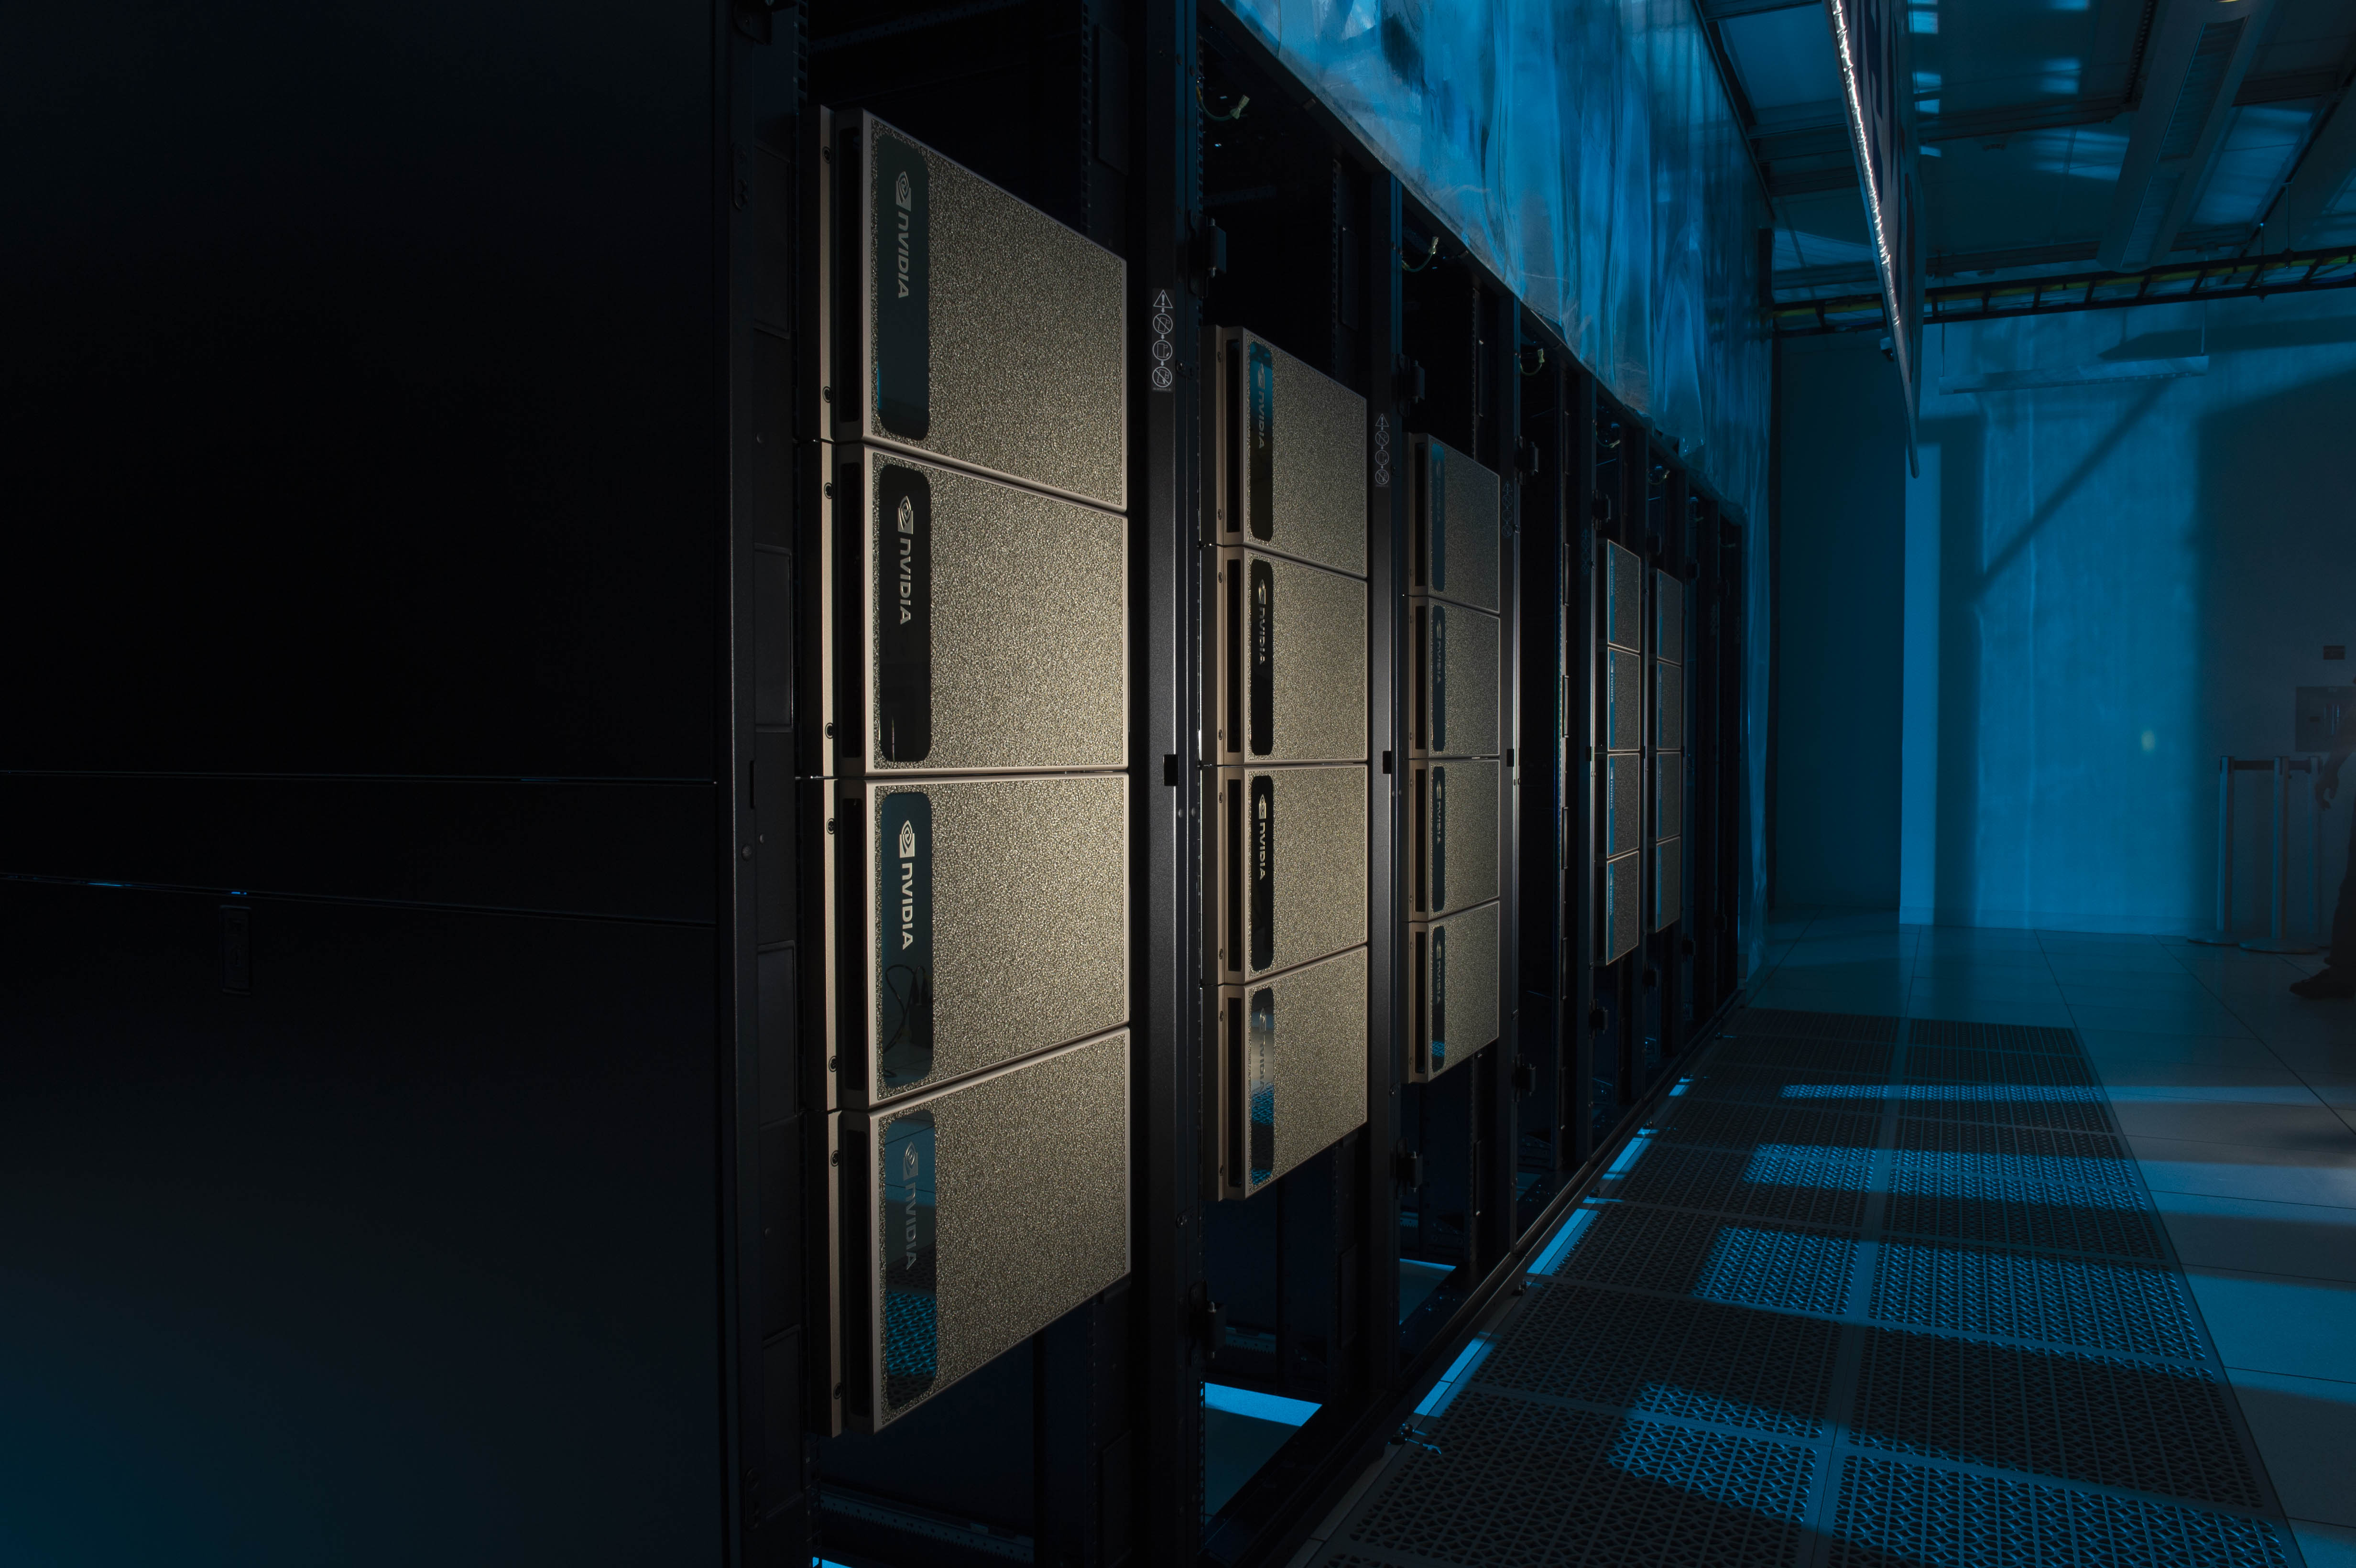
\includegraphics[width=0.85\textwidth]{images/superpod.jpg}}
\end{column}
\end{columns}
\end{frame}

\begin{frame}{Support}
\small
\begin{columns}[t]
\begin{column}{0.5\textwidth}
\href{https://southernmethodistuniversity.github.io/hpc\_docs/}{HPC Documentation}\newline\newline
\frame{
\includegraphics[width=0.8\textwidth]{images/hpc_docs_qr.png}}
\end{column}
\begin{column}{0.5\textwidth}
\href{https://libcal.smu.edu}{Help Sessions \& Workshops}\newline\newline
\frame{
\includegraphics[width=0.8\textwidth]{images/libcal_qr.png}}
\end{column}
\end{columns}
\end{frame}

\begin{frame}{Migration}
\centering
\frame{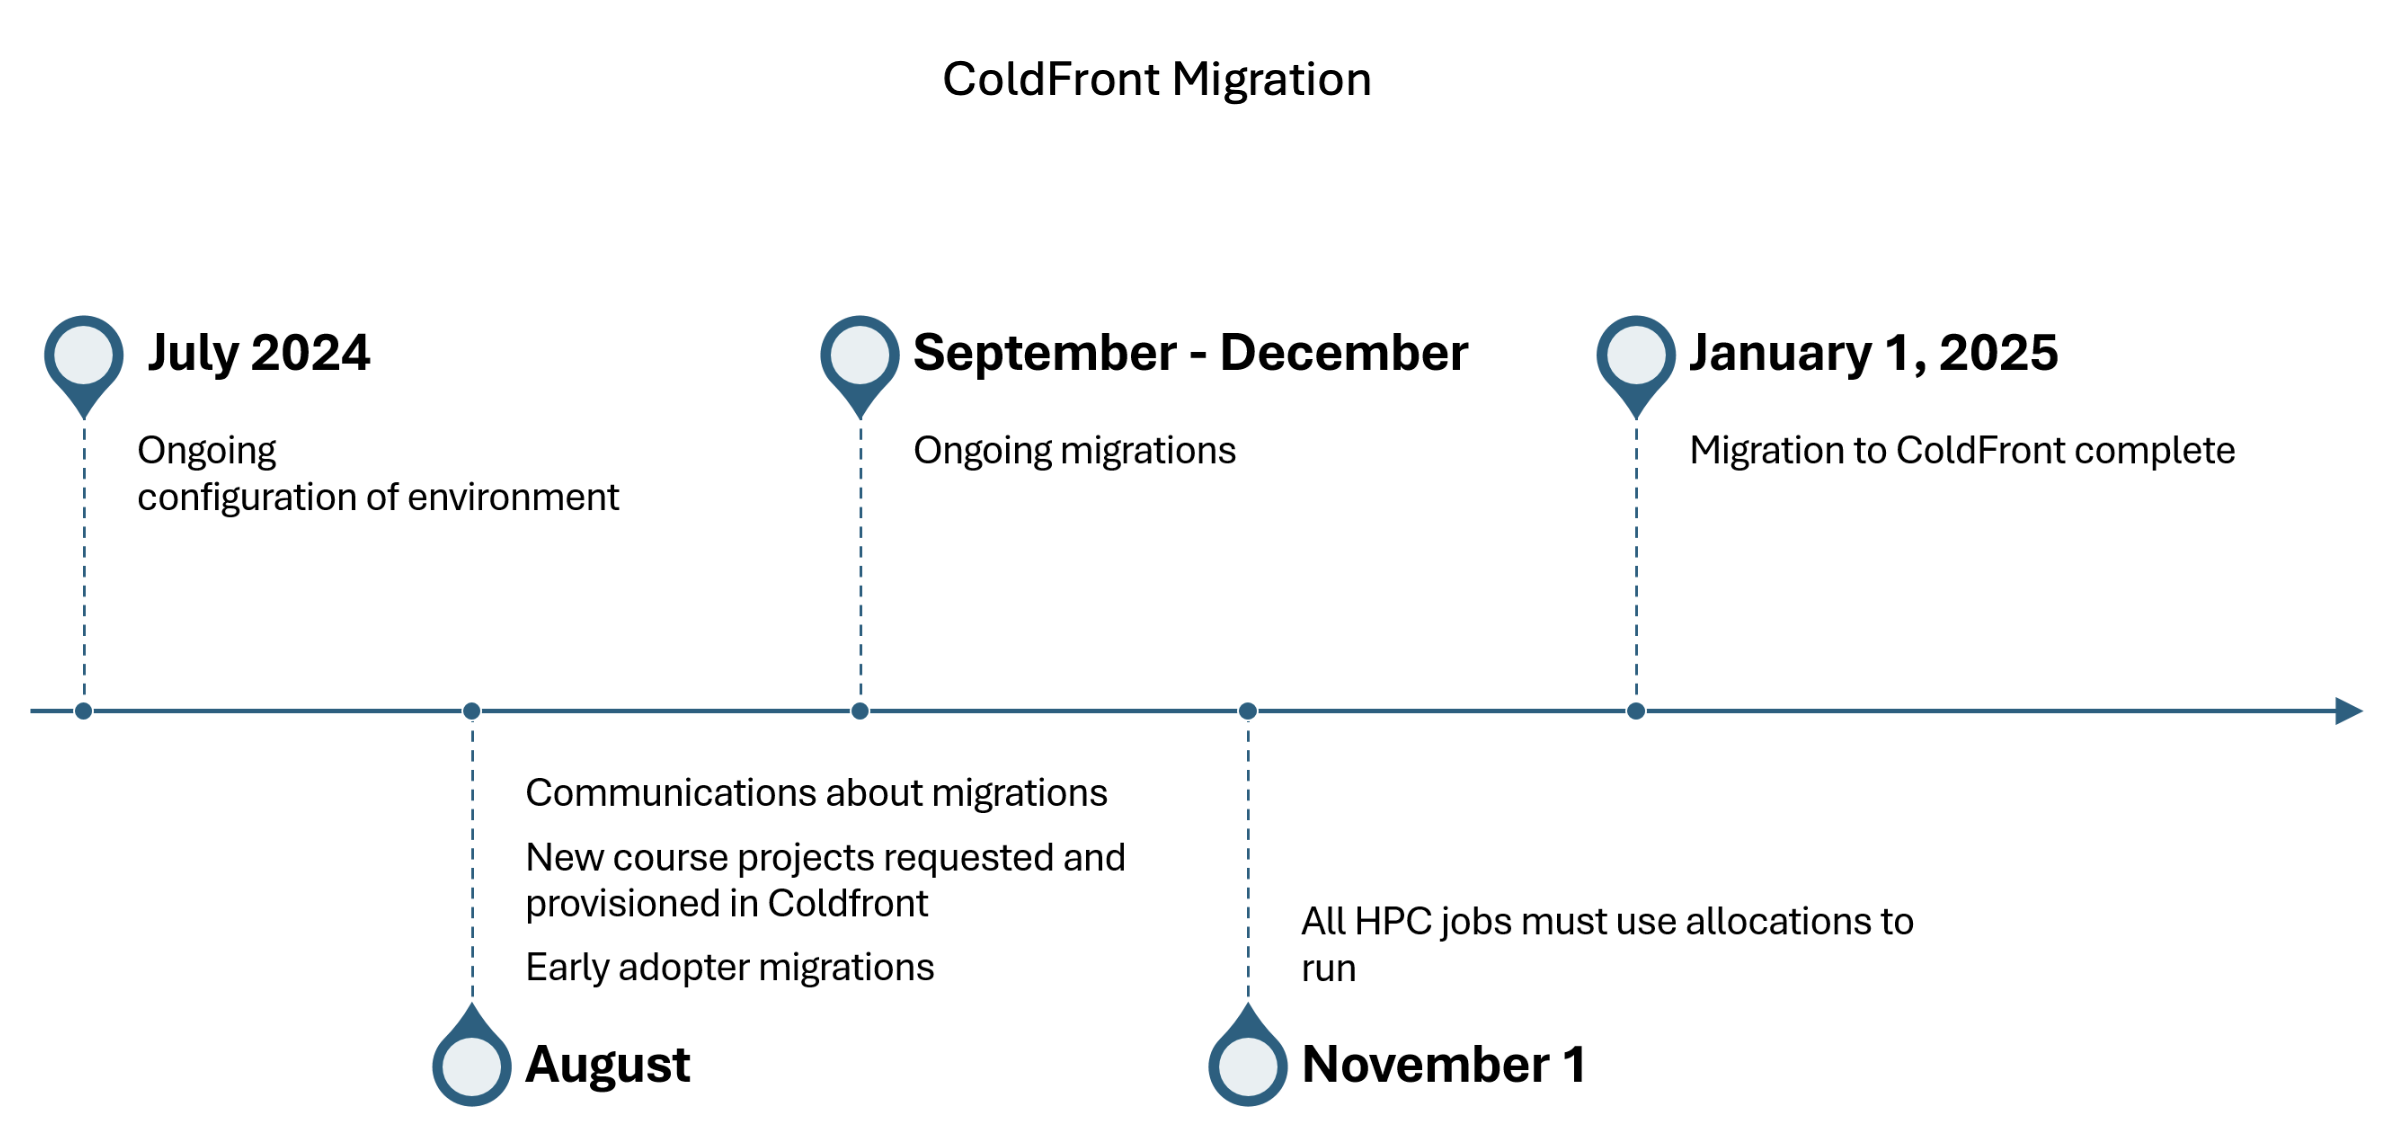
\includegraphics[width=0.9\textwidth]{images/coldfront_migration.png}}
\end{frame}

\section{Demo}

\section{Questions \& Discussion}

{
\setbeamertemplate{background}{
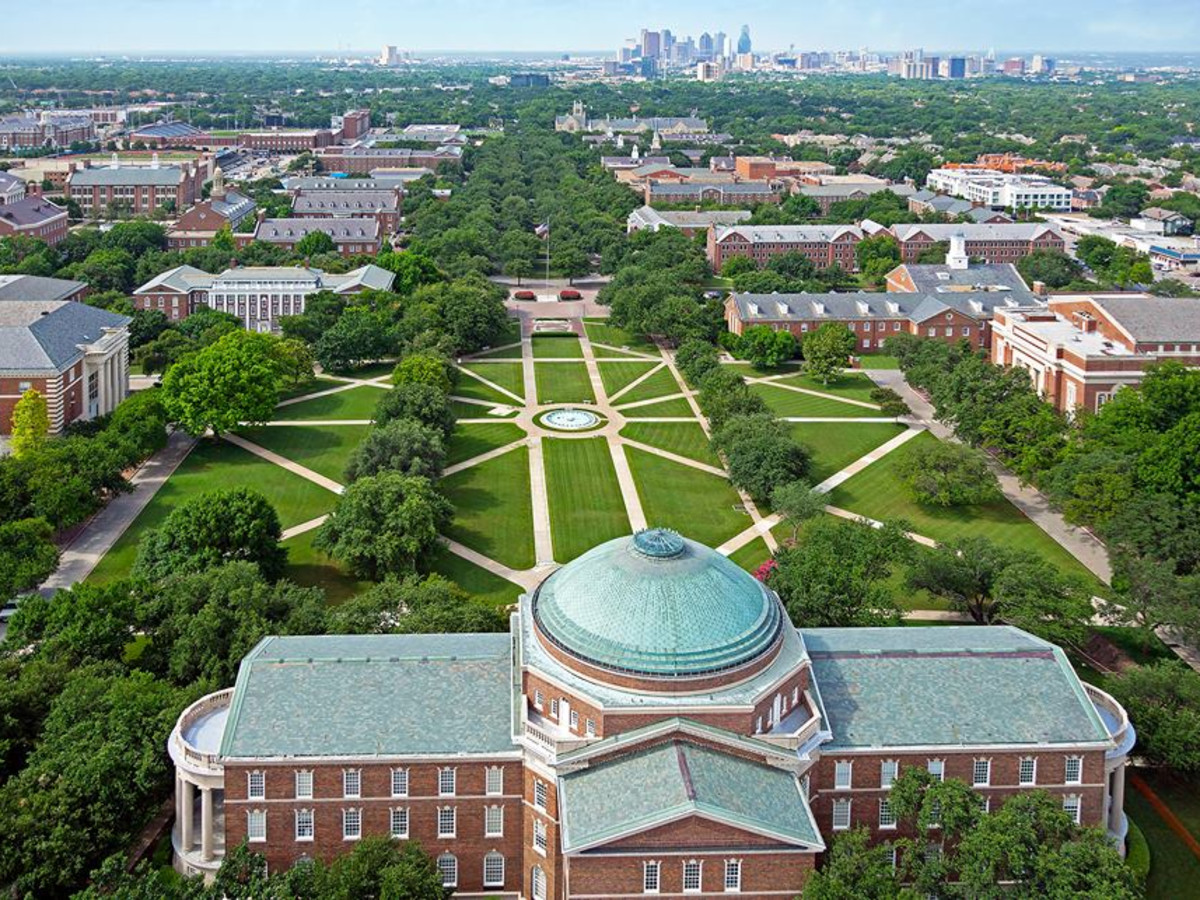
\includegraphics[width=\paperwidth,height=\paperheight]{images/smu_dallas.jpg}}
\begin{frame}
\begin{mybox}
\centering
\Huge
{\color{white}\textbf{Thank you!}}
\end{mybox}
\end{frame}
}

\end{document}

